\section{System Components}
In this section, we delve into the various components that make up the AAS Type3 system architecture. Each component is described in terms of its functionality, interactions with other components, and its role within the overall system.

\subsection{Resource Agent Components}

\begin{figure}[ht]
    \centering
    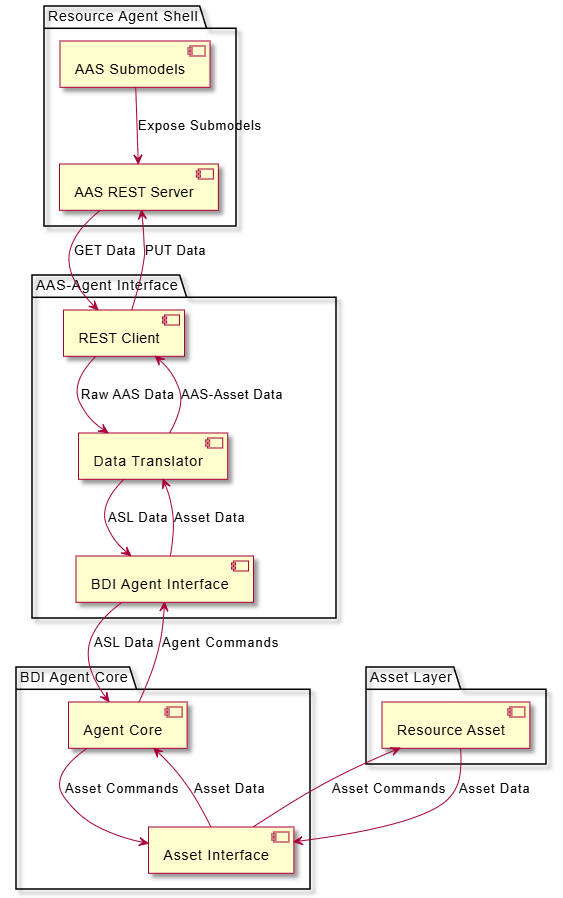
\includegraphics[width=0.7\textwidth]{Images/Resource_agent_components.png}
    \caption{Resource Agent Components Diagram}
    \label{fig:resource_agent_components}
\end{figure}

As illustrated in Figure \ref{fig:resource_agent_components}, the Resource Agent is composed of several key components over the layers that was discussed in the previous section.
In the first layer that is the \textbf{Resource Agent Shell}, it contains the following components:
\begin{itemize}
  \item \textbf{AAS Submodels} : those are the submodels of the AAS that describe the resource properties and capabilities.
  in which a Java server is used to host the AAS and provide access to its submodels.
  The server stores the AAS data into a database MongoDB for efficient retrieval and management.
  The AAS are mainly Json files that follow the AAS specification.
  \item \textbf{REST API server} : this component provides a RESTful interface for communication between the AAS and other system components.
  The Basyx framework provides this REST API server that allows clients to interact with the AAS submodels.
  The REST API server is a part of the Java server that hosts the AAS.
  It also opens MQTT communication channels for pub/sub messaging for real-time data exchange on update , create and delete operations on the AAS submodels. 
\end{itemize}

In the second layer that is the \textbf{AAS-Agent Interface layer}.
This layer as discussed before is responsible for the communication between the AAS and the Agent.
The layer contains three main components:
\begin{itemize}
  \item \textbf{REST Client} : This is the main layer for communication between the Agent and the AAS.
  Which is responsible for sending requests to the AAS REST API server and receiving responses.
  This client shall allow the Agent to read , write and deleted information about the asset, submodels and the submodels elements.
  \item \textbf{Data Translator} : This is the core component of the AAS-Agent interface layer.
  It is responsible for translating the data between the AAS format and the Agent's internal data structures.
  Where it takes raw data from the AAS and converts them into a format that the Agent can understand and vice versa.
  \item \textbf{BDI Agent Interface }: This component acts as a bridge between the Data Translator and the BDI Agent.
  It ensures that the translated data is properly integrated into the Agent's belief, desire, and intention structures.
  It also facilitates the communication of the Agent's decisions and actions back to the AAS through the Data Translator.
\end{itemize}
The last layer is the \textbf{BDI Agent Core} layer.
This layer contains the main components of the BDI Agent architecture:
\begin{itemize}
  \item \textbf{Agent Core} : This is the central component of the BDI Agent.
  It manages the Agent's beliefs, desires, and intentions.
  It processes incoming data from the AAS and makes decisions based on its internal state and goals.
  It also procees data coming from the Resource Asset it is assigned to manage.
  The main functionality is update beliefs based on the data received from the AAS and the Resource Asset.
  Then it generates desires and intentions based on the updated beliefs and the Agent's objectives.
  \item \textbf{Asset Interface} : This component is responsible for communication between the BDI Agent and the Resource Asset.
  It contains the necessary protocols and methods to interact with the asset, retrieve data, and send commands.
\end{itemize}

\newpage
\subsection{Production Agent Components}

\begin{figure}[ht]
    \centering
    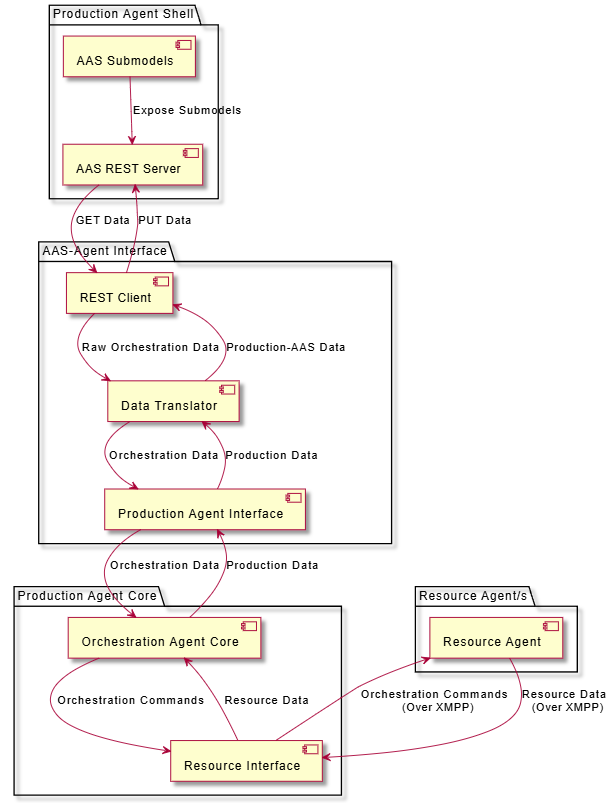
\includegraphics[width=0.8\textwidth]{Images/Production_Agent_Components.png}
    \caption{Production Agent Components Diagram}
    \label{fig:production_agent_components}
\end{figure}

The Production Agent components are illustrated in Figure \ref{fig:production_agent_components}.
It has similar structure to the Resource Agent components with some differences in the Agent Core layer and the AAS-Agent Interface layer.
In the \textbf{AAS-Agent Interface layer}, the components are similar to the Resource Agent with the data translator being adapted to handle production-specific data from the AAS submodels.
This includes translating production schedules, work orders, and status updates between the AAS format and the Agent's internal structures.
The AAS-Agent Interface gets the Raw orchestration commands from the Production AAS where it then translates them into an orchestration command
that the orchestration core can understand and act upon.
At the same time the data coming from the Production Agent core about the production status and progress is translated back into the AAS format and updated into the Production AAS submodels.

In the main layer that is the \textbf{Production Agent core} layer the diffrences are more significant.
The Production Agent core contains the \textbf{orchestration agent core } component instead of the BDI agent core.
This component is responsible for managing the orchestration of production tasks and workflows.
It processes orchestration commands received from the AAS-Agent interface layer and coordinates the execution of these
tasks across multiple Resource Agents and assets.
It also monitors the progress of production activities and updates the AAS with status information through the AAS-Agent interface layer.
The \textbf{Resource Interface} component in this layer is also adapted
to handle communication with production-related assets, such as manufacturing equipment and assembly lines.
It ensures that the Production Agent can effectively manage and control these assets as part of the overall production process.

